\graphicspath{{./figures/}}
\title{}
\date{}
\usepackage{pgfpages}
\begin{document}
\begin{frame}
    \titlepage
\end{frame}

\begin{frame}{last time (1)}
    \begin{itemize}
    \item CHALLENGE logistics
    \item the system call interface is big:
        \begin{itemize}
        \item hard to enumerate needed system calls
        \item easy to miss features (e.g. runc bug) that need to be restricted
        \end{itemize}
    \item isolating programs that used shared services (e.g. windowing service)
        \begin{itemize}
        \item proxy? another system-call like interface?
        \end{itemize}
    \end{itemize}
\end{frame}

\begin{frame}{last time (2)}
    \begin{itemize}
    \item mandatory access control, example: SELinux
        \begin{itemize}
        \item ``type'' labels for objects (files, etc.)
        \item explicit list of allowed operations
        \item enforcement in OS
        \end{itemize}
    \item separate views of system resources for sandboxes
        \begin{itemize}
        \item chroot: program views subset of filesystem
        \item mount namespace: independent view of available disks
            \begin{itemize}
            \item ``bind mounts'' to expose directory `outside' as virtual disk
            \end{itemize}
        \item pid, network, etc. namespaces --- container $\approx$ lightweight VM sharing OS
        \end{itemize}
    \end{itemize}
\end{frame}

\subsubsection{runC bug}
\begin{frame}{runc bug}
    \begin{itemize}
    \item 2019 bug in Docker, other container implementations (CVE-2019-5736)
        \begin{itemize}
        \item blog post for vulnerability finders: \\\scriptsize \url{https://blog.dragonsector.pl/2019/02/cve-2019-5736-escape-from-docker-and.html}
        \end{itemize}
    \vspace{.5cm}
    \item bug setup:
        \begin{itemize}
        \item user starts malicious container X
        \item user tells docker to start a new command in malicious container X
        \item \myemph<2>{malicious container X hijacks the ``new command'' starting program}
        \item hijacked program used to access stuff outside container
        \end{itemize}
    \item part of problem: Docker and others weren't using user namespaces at the time
        \begin{itemize}
        \item compatability problems
        \end{itemize}
    \end{itemize}
\end{frame}

\begin{frame}{setup: /proc/PID}
    \begin{itemize}
    \item Linux provides /proc directory to access info about programs
    \item used for implementing process list utils, debugging
        \begin{itemize}
        \item needed to make a functional container
        \end{itemize}
    \item subdirectory for each process in current container
        \begin{itemize}
        \item process ID PID has /proc/PID subdirectory
        \item /proc/self is alias for current process's subdirectory
        \end{itemize}
    \vspace{.5cm}
    \item included is /proc/PID/exe file --- alias for executable file
    \end{itemize}
\end{frame}

\begin{frame}{running a command in existing container}
    \begin{itemize}
    \item to run command X in existing container:
    \vspace{.5cm}
    \item step 1: switch current process to that container
    \item<2-> \myemph{code in container can access /proc here?}
    \item<2-> \myemph{including overwriting /proc/self/exe!}
        \begin{itemize}
        \item which is a program run as root!
        \end{itemize}
    \vspace{.25cm}
    \item step 2: execute command X
    \end{itemize}
\end{frame}


\begin{frame}{partial fix}
    \begin{itemize}
    \item can disable access to /proc/PID/exe (and related things)
    \item system call: \texttt{prctl(PR\_SET\_DUMPABLE, 0)}
    \item but\ldots the run-in-container tool did this for a while
    \vspace{.5cm}
    \item<2-> problem: this gets reset on executing a new program
    \item<2-> and attacker could make the new program be /proc/PID/exe
        \begin{itemize}
        \item one mechanism: symbolic links (file aliases)
        \end{itemize}
    \item<2-> but change dynamic linking setup to run attacker code
    \item<2-> \ldots which accesses /proc/self/exe
    \end{itemize}
\end{frame}

\begin{frame}{full fix}
    \begin{itemize}
    \item make single-use copy of start-in-container tool each time command run
        \begin{itemize}
        \item in-memory file
        \end{itemize}
    \item \ldots so modifying it doesn't change anything
        \begin{itemize}
        \item (but it's also protected from modification)
        \end{itemize}
    \vspace{.5cm}
    \item other solutions:
        \begin{itemize}
        \item make executable non-writable (e.g. SELinux, don't run container as root)
        \end{itemize}
    \end{itemize}
\end{frame}


\subsection{SELinux sandbox escape}
\begin{frame}{SELinux escape}
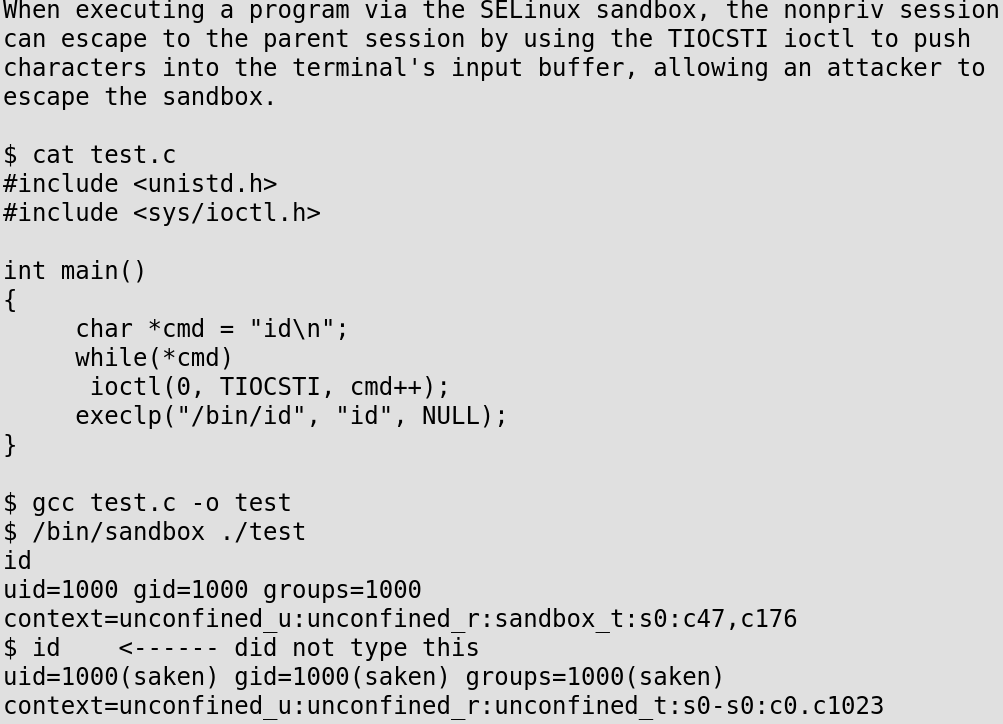
\includegraphics[height=0.9\textheight]{../sandbox/selinux-escape-email}
\end{frame}

\section{the Android sandbox}
\begin{frame}{Android sandbox}
    \begin{itemize}
    \item Android --- Linux based OS for phones/tablets
    \vspace{.5cm}
    \item \url{https://source.android.com/security/app-sandbox}
    \item current version: SELinux + seccomp (system call filter)
    \end{itemize}
\end{frame}


% FIXME: Android sandbox

\subsection{OSX sandboxing}

\begin{frame}{OS X sandboxing}
    \begin{itemize}
    \item OS X (tries to) implement system call filtering
    \item main challenge: what about files?
        \begin{itemize}
        \item user can open a file anywhere --- we expect that to work
        \end{itemize}
    \item<2> OS X solution: OS service displays file-open dialog
        \begin{itemize}
        \item OS knows user really choose a file
        \end{itemize}
    \item<2> application can ask to remember file was chosen previously
    \item<2> not chosen/remembered --- can't access
        \begin{itemize}
        \item requires changes to how applications open files
        \end{itemize}
    \end{itemize}
\end{frame}


\subsection{Qubes}

\begin{frame}{another sandboxing OS: Qubes}
    \begin{itemize}
    \item Qubes: heavily sandboxed OS
    \item runs \myemph{seperate VMs} instead of filtering syscalls
    \item UI that clearly shows what VM each window is from
    \vspace{.5cm}
    \item advantage: easier to gaurentee isolation
        \begin{itemize}
        \item many, many more bugs in system call filtering than VMs
        \end{itemize}
    \item disadvantage: harder to share between VMs
    \item disadvantage: much more runtime overhead
    \end{itemize}
\end{frame}

\begin{frame}{Qubes screenshot}
    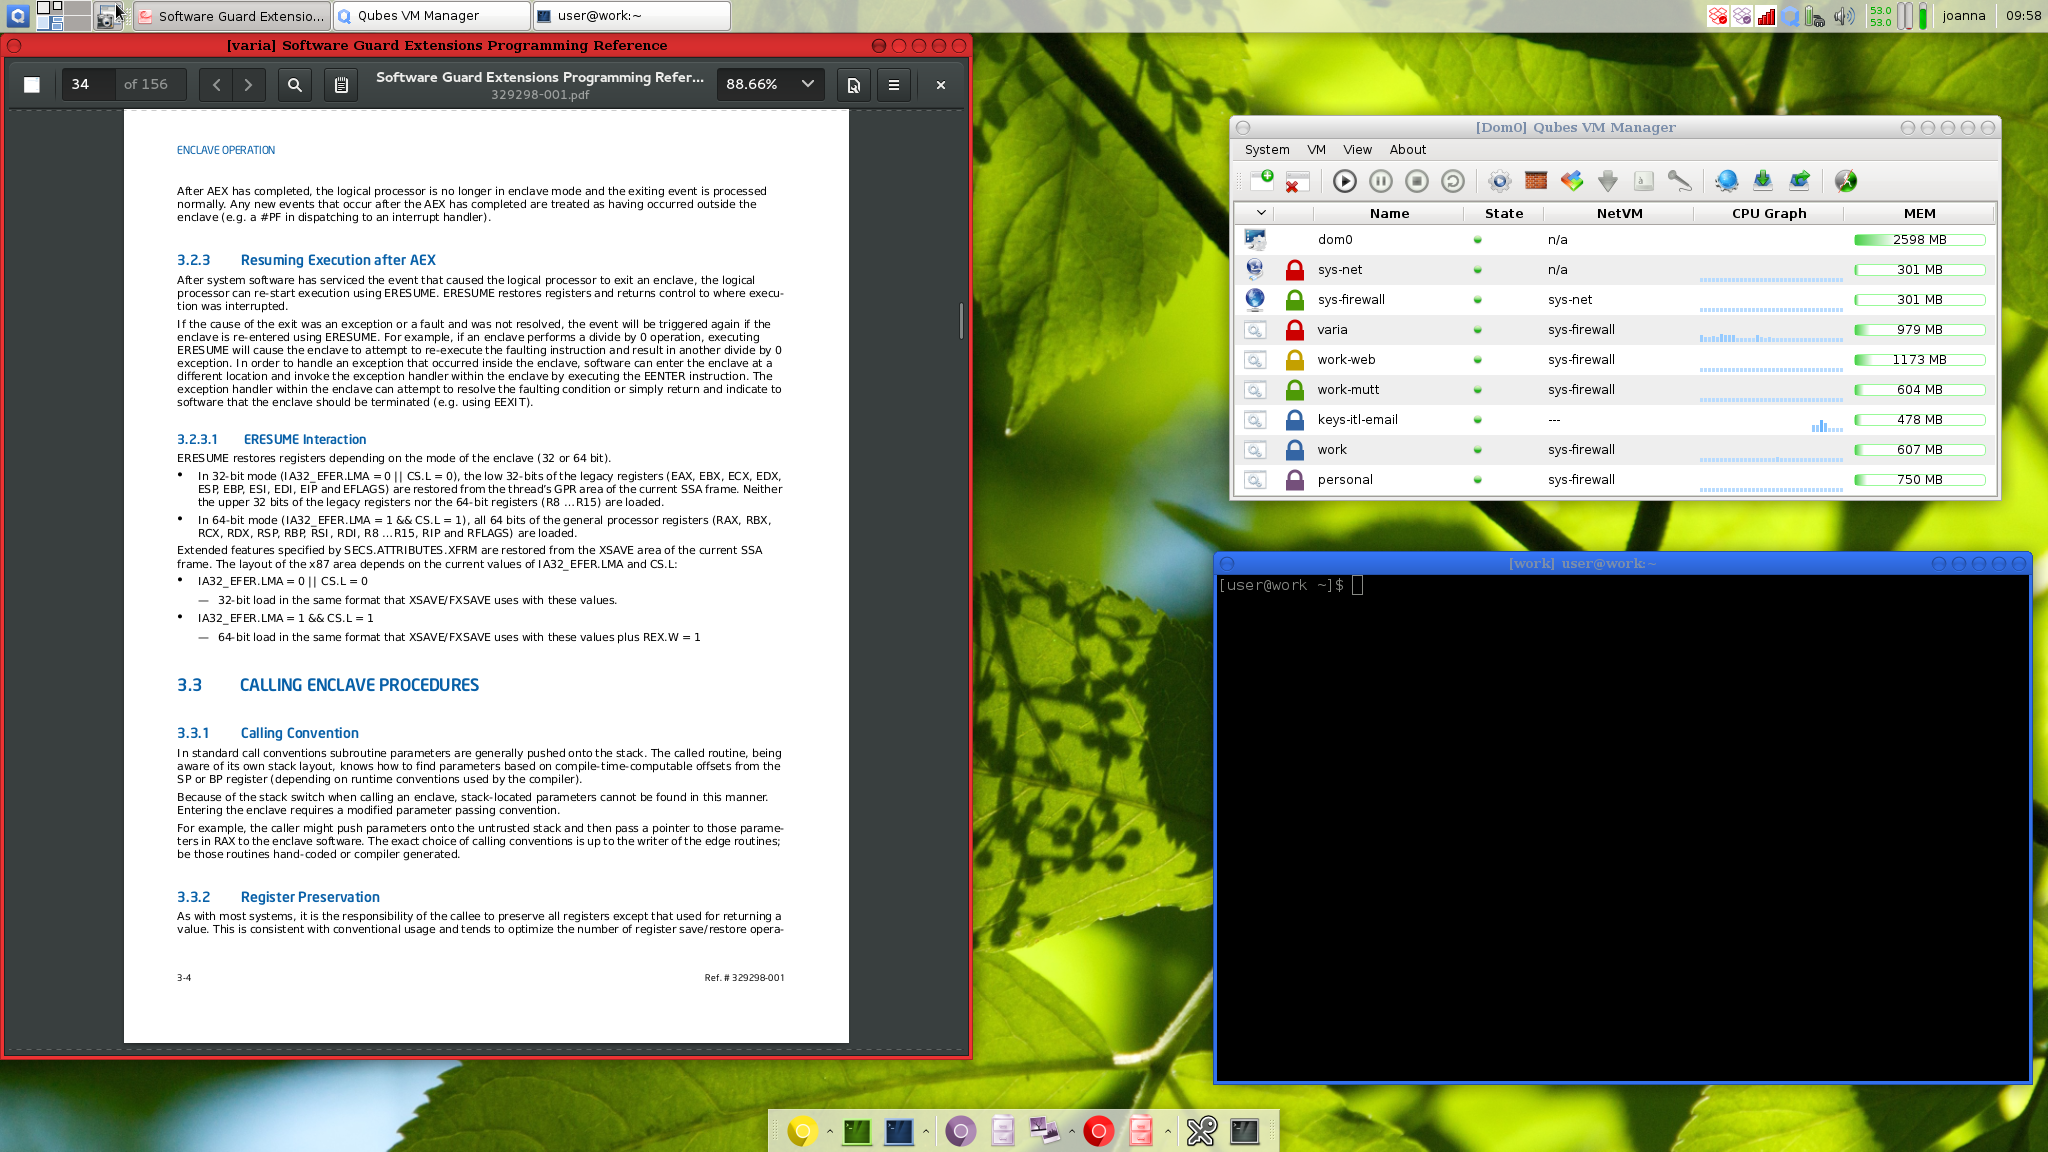
\includegraphics[width=\textwidth]{../sandbox/qubes-desktop1}
\end{frame}




\section{Which sandboxing?}
\begin{frame}{which sandboxing?}
    \begin{itemize}
    \item which whole-application sandboxing technique seems better for 
        \begin{itemize}
        \item security, performance, usability, handling unchanged applications
        \end{itemize}
    \item (full answer: could mix techniques + probably depends on details of app)
    \vspace{.5cm}
    \item A. chroot + system call filtering
    \item B. chroot + mount and user namespaces
    \item C. virtual machine dedicated to application
    \item D. SELinux-like mandatory access control
    \end{itemize}
\end{frame}


\section{sandboxing without OS support}
\begin{frame}{sandboxing without OS support}
    \begin{itemize}
    \item so far: relying on OS features for sandboxing
    \item good reasons:
        \begin{itemize}
        \item primarily want to filter system calls
        \item hardware-assisted, strong protection
        \end{itemize}
    \vspace{.5cm}
    \item but problems with relying on OS:
        \begin{itemize}
        \item sending information in/out of sandbox relatively slow
        \item requires heavily OS-specific code
        \end{itemize}
    \end{itemize}
\end{frame}

\begin{frame}{sandboxing without OS ideas}
    \begin{itemize}
    \item `dynamic' language virtual machine, like Java VM, .Net CLR
        \begin{itemize}
        \item hard to use with code intended to compile to native machine code
        \end{itemize}
    \vspace{.5cm}
    \item virtual machine targetted for C/C++-like code, like WebAssembly
    \vspace{.5cm}
    \item assembly-to-assembly conversion
        \begin{itemize}
        \item example: Wahbe, Lucco, Anderson, and Graham, ``Efficient Software-Based Fault Isolation'' (1993)
        \item example: Ford and Cox, ``Vx32: Lightweight User-level Sandboxing on the x86'' (2008)
        \end{itemize}
    \end{itemize}
\end{frame}


\subsection{Wasm}
\begin{frame}{WebAssembly}
    \begin{itemize}
    \item WebAssembly: language virtual machine specification intended\ldots
        \begin{itemize}
        \item similar idea to Java VM
        \end{itemize}
    \vspace{.5cm}
    \item to be compiled to from C/C++
        \begin{itemize}
        \item support by Clang/LLVM
        \end{itemize}
    \item to be easy to just-in-time compile to native machine code
    \item to be run in web browsers (fast web apps)
    \end{itemize}
\end{frame}

\begin{frame}{WebAssembly memory management}
    \begin{itemize}
    \item WebAssembly `modules' have a single ``linear memory''
    \item starts at index 0, goes to some maximum
    \item load/store instructions take index into current memory
    \vspace{.5cm}
    \item observation 1: close to memory model ``normal'' C/C++ code expects
    \vspace{.5cm}
    \item observation 2: only goal is to prevent sandbox (WebAssembly) code from interfering with outside code
    \item \ldots so no need to check array bound or similar
    \vspace{.5cm}
    \item observation 3: no need to worry about garbage collection
    \end{itemize}
\end{frame}

\begin{frame}{WebAssembly validation}
    \begin{itemize}
    \item WebAssembly virtual machine code designed to be \textit{validated} before running
    \vspace{.5cm}
    \item allows for efficient interpreters or conversion to assembly
        \begin{itemize}
        \item validation ensures that you can safely skip certain type checks, etc.
        \end{itemize}
    \item language specification very explicit about what needs to be checked at runtime
    \end{itemize}
\end{frame}

\begin{frame}{example WebAssembly validation}
    \begin{itemize}
    \item check that instructions have right number of operands available
        \begin{itemize}
        \item WebAssembly instructions use stack (compile \texttt{2 + 2} into \texttt{2 2 +})
        \end{itemize}
    \item check operands that can be checked (constants)
    \item check the calls go to only functions listed in table
        \begin{itemize}
        \item should make it easier to do just-in-time compilation to machine code?
        \end{itemize}
    \item check the branches go to only locations listed in table, and only within one function
        \begin{itemize}
        \item should make it easier to do just-in-time compilation to machine code?
        \end{itemize}
    \end{itemize}
\end{frame}

\begin{frame}{example WebAssembly instruction specification}
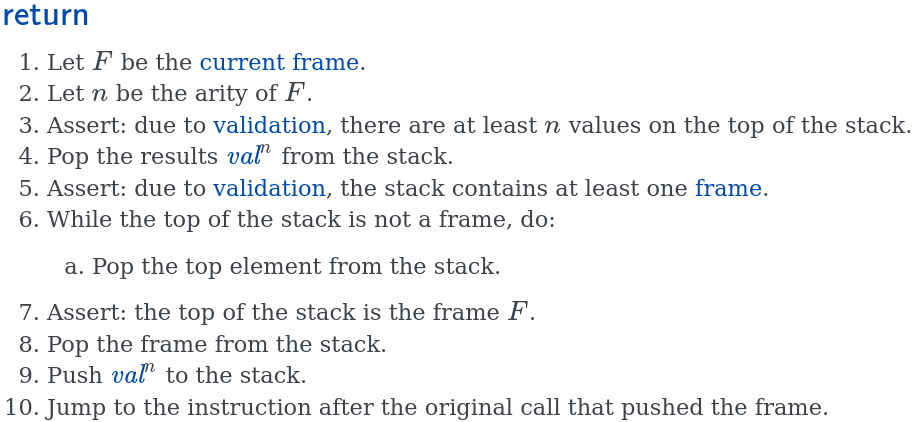
\includegraphics[height=0.8\textheight]{../sandbox/wasm-return-spec}
\end{frame}

\begin{frame}{WebAssembly as sandboxing}
    \begin{itemize}
    \item can compile existing C/C++ library using WebAssembly\ldots
    \item then call using language virtual machine
    \end{itemize}
\end{frame}



\section{sandboxing API: RLBox}
\begin{frame}{RLBox}
    \begin{itemize}
    \item saw interfaces for using sandboxes from user perspective?
    \item what about for privilege separation?
        \begin{itemize}
        \item recall: like Chrome separate renderer process idea
        \item need to navigate OS sandboxing API + create interface for sandboxed part?
        \end{itemize}
    \vspace{.5cm}
    \item some reusable tools have appeared for this (but no clear winner)
    \item one example: RLBox (published in Usenix Security 2020)
        \begin{itemize}
        \item Shravan Narayan and Craig Disselkoen, UC San Diego; Tal Garfinkel, Stanford University; Nathan Froyd and Eric Rahm, Mozilla; Sorin Lerner, UC San Diego; Hovav Shacham, UT Austin; Deian Stefan, UC San Diego
        \end{itemize}
    \end{itemize}
\end{frame}

\begin{frame}[fragile,label=rlboxusage]{RLBox usage}
\begin{itemize}
\item part of example from author's presentation:
    \begin{itemize}
    \item goal: invoke JPEG parser in sandbox
    \end{itemize}
\end{itemize}
\begin{lstlisting}[language=C++,style=script]
autosandbox = rlbox::create_sandbox<wasm>();
tainted<jpeg_decompress_struct*> p_jpeg_img = sandbox.malloc_in_sandbox<jpeg_decompress_struct>();
tainted<jpeg_source_mgr*> p_jpeg_input_source_mgr = sandbox.malloc_in_sandbox<jpeg_source_mgr>();
sandbox.invoke(jpeg_create_decompress, p_jpeg_img);
p_jpeg_img->src = p_jpeg_input_source_mgr;
p_jpeg_img->src->fill_input_buffer = ...;
sandbox.invoke(jpeg_read_header,p_jpeg_img/*...*/);
\end{lstlisting}
\begin{itemize}
\item tool handles running `jpeg\_create\_decompress', `jpeg\_read\_header' in sandbox
\item values shared with sandbox marked as ``tainted''
    \begin{itemize}
    \item C++ (template) class
    \end{itemize}
\item this example: using WebAssembly-based sandbox
\item used in firefox
\end{itemize}
\end{frame}


\section{application permissions}
\usetikzlibrary{calc}
\begin{frame}{some Android prompts}
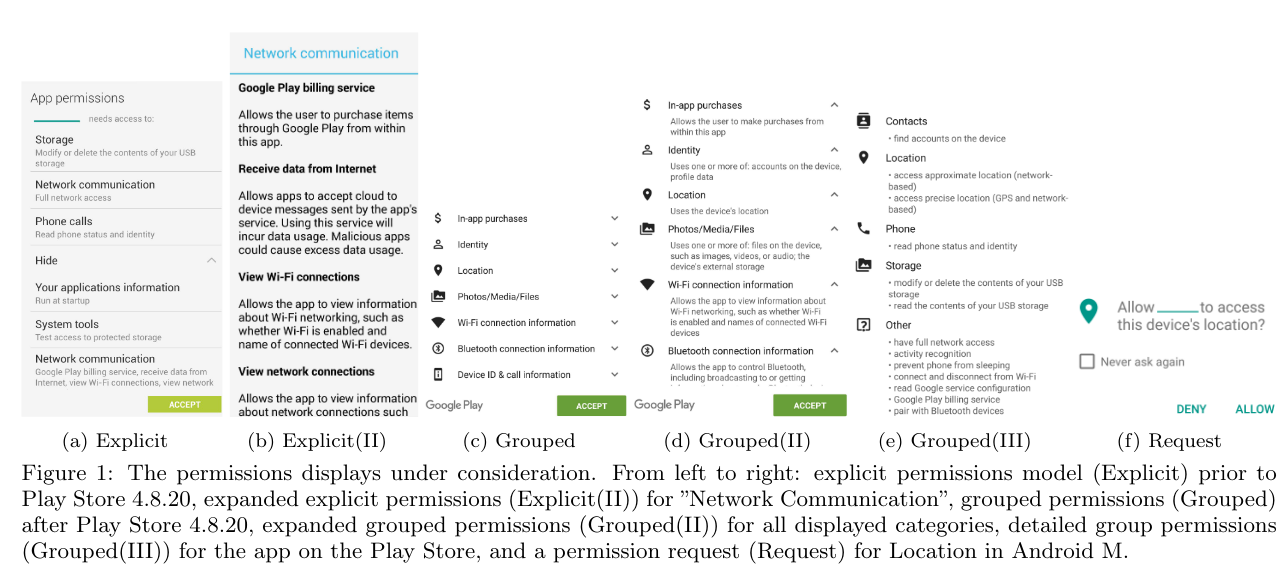
\includegraphics[width=\textwidth]{../sandbox/android-perm-screens}
\imagecredit{from Clark et al, ``No Time At All: Opportunity Cost of Android Permissions'' (HotWireless'16)}
\end{frame}


\subsection{UI problems}

\begin{frame}<1>[label=appPermUI]{UI problems with application permissions}
    \begin{itemize}
    \item \myemph<2>{do applications request sensible permissions?}
    \item \myemph<3>{do users pay attention to permission requests?}
    \item \myemph<3>{do users understand what permissions mean?}
    \item are permissions fine-grained enough?
    \item are permissions coarse-grained enough?
    \end{itemize}
\end{frame}


\subsection{do request right permissions?}
\againframe<2>{appPermUI}
\begin{frame}{right permissions?}
    \begin{itemize}
    \item Felt, Chin, Hanna, Song and Wagner, ``Android Permissions Demystified'' (CCS 2011)
    \item used static analysis to compare requested permissions to what applications did
        \begin{itemize}
        \item at the time: permissions requested at installation
        \end{itemize}
    \item sample of 900 applications
    \item estimate approx 200 over-privileged
        \begin{itemize}
        \item (estimate because using false positive rate from manual checking)
        \end{itemize}
    \end{itemize}
\end{frame}

\begin{frame}{why extra permissions?}
    \begin{itemize}
    \item selected from Felt et al's analysis:
    \item developers confused similar permissions
        \begin{itemize}
        \item \texttt{ACCESS\_NETWORK\_STATE} versus \texttt{ACCESS\_WIFI\_STATE}
        \end{itemize}
    \item developers thought permissions were needed for delegated tasks
        \begin{itemize}
        \item \texttt{CALL\_PHONE} not needed to invoke phone app
        \item \texttt{INSTALL\_APPLICATION} not needed to open app store install dialog
        \end{itemize}
    \item developers thought permissions needed for all methods of class
        \begin{itemize}
        \item \texttt{WRITE\_SETTINGS} when using (no-permission) read-settings operations
        \end{itemize}
    \item copy-and-paste
    \end{itemize}
\end{frame}


\subsection{do users understand permissions?}
\againframe<3>{appPermUI}
\begin{frame}{a user study (2012)}
    \begin{itemize}
    \item Felt, Ha, Egelman, Haney, Chin, Wagner, ``Android Permissions: User Attention, Comprehension, and Behavior''
    \item performed lab study; task: find + install coupon app
    \item at the time: Android prompted for permissions on installation
    \vspace{.5cm}
    \item<2-> 17\% looked at app permissions detail
    \item<2-> 42\% aware of permissions
    \item<2-> 42\% unaware of permissions
    \vspace{.5cm}
    \item<2-> versus: 88\% read reviews 
    \end{itemize}
\end{frame}

\begin{frame}{a user survey (2012)}
    \begin{itemize}
    \item same paper did survey about what permissions meant
    \item three multiple choice questions 
        \begin{itemize}
        \item selected from bank of 11
        \end{itemize}
    \item 302 respondents; 3 fully correct
    \item average 21\%
    \end{itemize}
\end{frame}

\begin{frame}{example survey question}
    \begin{itemize}
    \item `Read phone state and identity' allows which of these?
    \vspace{.5cm}
    \item Read your phone number
    \item See who you have called
    \item Track you across applications
    \item Load adverisements
    \end{itemize}
\end{frame}

\begin{frame}{survey questions (1)}
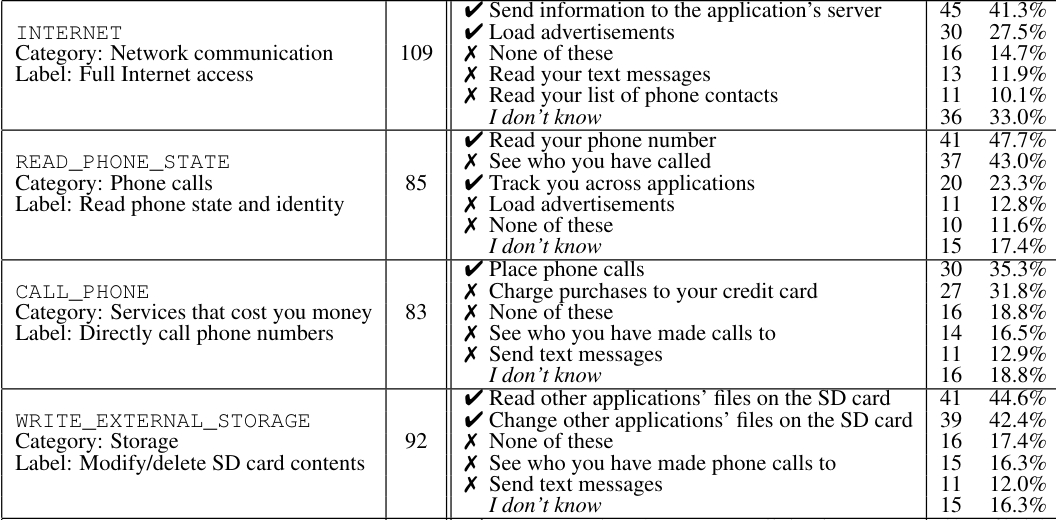
\includegraphics[width=\textwidth]{../sandbox/android-perm-survey1}
\end{frame}

\begin{frame}{survey questions (2)}
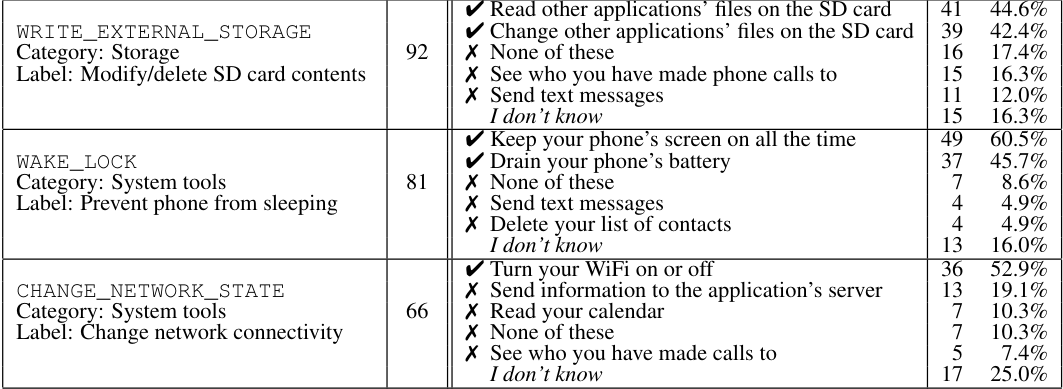
\includegraphics[width=\textwidth]{../sandbox/android-perm-survey2}
\end{frame}

\begin{frame}{survey questions (3)}
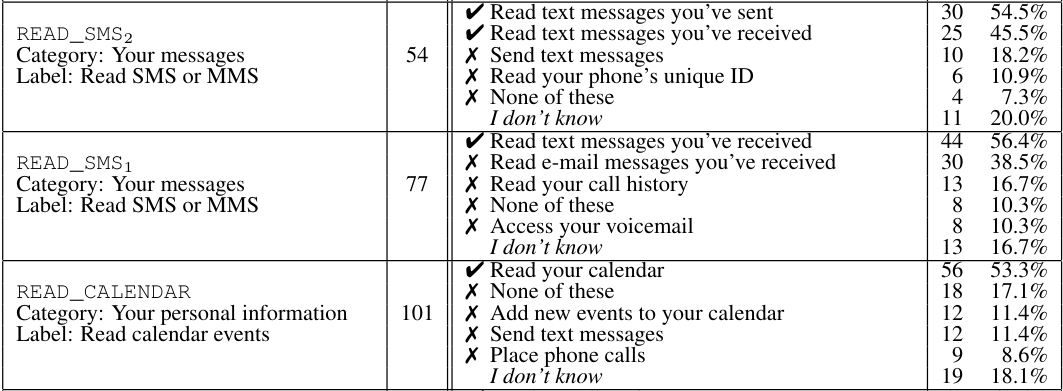
\includegraphics[width=\textwidth]{../sandbox/android-perm-survey3}
\end{frame}

\begin{frame}{survey questions (4)}
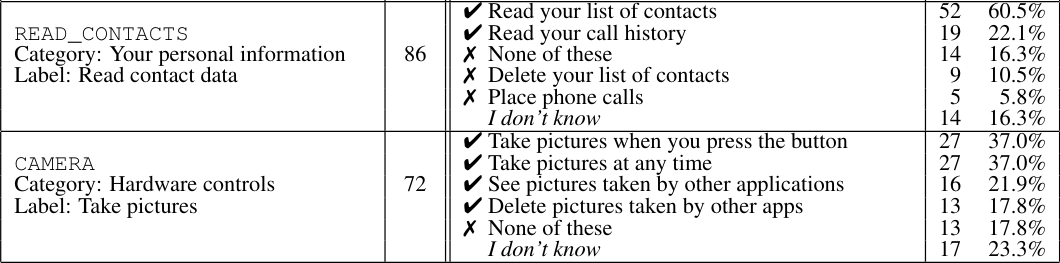
\includegraphics[width=\textwidth]{../sandbox/android-perm-survey4}
\end{frame}


\subsection{how to ask for permission?}
\begin{frame}
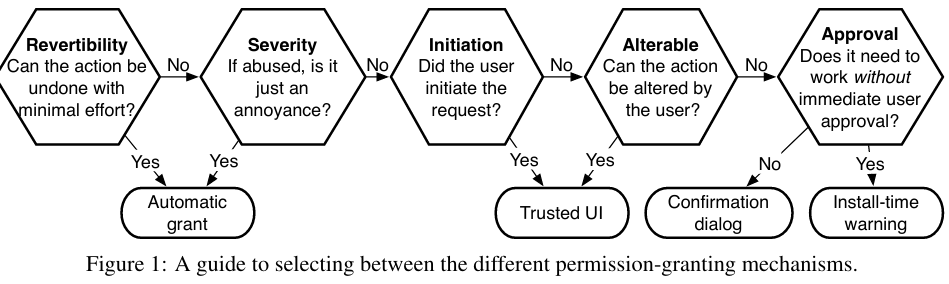
\includegraphics[width=\textwidth]{../sandbox/app-perm-how}
\scriptsize from Felt et al, ``How To Ask For Permission'' (HotSec'12)
\end{frame}

\begin{frame}{principles}
    \begin{itemize}
    \item Felt et al list ``principles'':
    \vspace{.5cm}
    \item ``Conserve user attention, utilizaing it for only permissions that have severe consquences''
        \begin{itemize}
        \item too many security warnings means users won't pay attention
        \end{itemize}
    \item ``When possible, avoid interrupting the user's primary task with explicit security decisions''
        \begin{itemize}
        \item users will dismiss warnings because they get in the way of work
        \end{itemize}
    \end{itemize}
\end{frame}


\subsection{permissions abuse: Cloak and Dagger}
\begin{frame}{Cloak and Dagger}

\includegraphics[width=\textwidth]{../sandbox/cloak-and-dagger}
\end{frame}

\begin{frame}{cloak and dagger permissions}
    \begin{itemize}
    \item the two permissions:
        \begin{itemize}
        \item SYSTEM\_ALERT\_WINDOW: \\
            draw windows on top of screen \\
            (at time: enabled by default)
        \item BIND\_ACCESSIBILITY\_SERVICE: \\
            ``Observe your actions'' \\
            ``Retrieve window content''
        \end{itemize}
    \item can hide window content while user interacts with it
    \item \ldots and stealthy get user to do more things
    \end{itemize}
\end{frame}

\begin{frame}{also, a clickjacking attack}
    \begin{itemize}
    \item at the time, could draw overlay window over permissions dialog
    \item \ldots convince user to press where ``OK'' button is
    \item countermeasure: permissions dialog would detect this, ignore clicks
    \vspace{.5cm}
    \item problem: wouldn't detect if overlay didn't cover enough of button
    \end{itemize}
\end{frame}


\subsection{permissions abuse: information leak}
\begin{frame}{privacy and permissions}
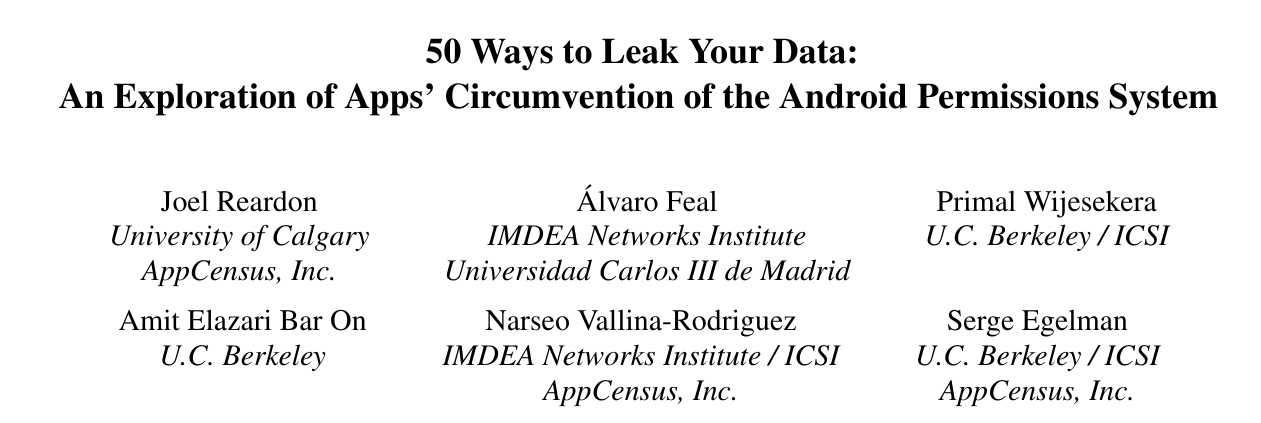
\includegraphics[width=0.7\textwidth]{../sandbox/priv-and-perm}
    \begin{itemize}
    \item 2019 paper
    \item many mobile application permissions related to privacy
    \item getting phone ID, email address, location, \ldots
    \item but applications (especially ad libraries) find workarounds
    \end{itemize}
\end{frame}

\begin{frame}{permissions being insufficient}
    \begin{itemize}
    \item permissions check limited API calls for getting private info,\ldots
    \item \ldots but there were alternative, unfiltered system calls for
    \vspace{.5cm}
    \item getting MAC address (effectively phone ID)
        \begin{itemize}
        \item Linux \texttt{ioctl} system call on socket
        \end{itemize}
    \item WiFi base station address
        \begin{itemize}
        \item ARP cache (recently seen machines on network, to know where to send packets)
        \end{itemize}
    \item location
        \begin{itemize}
        \item geolocation tag on recent photos
        \end{itemize}
    \end{itemize}
\end{frame}

\begin{frame}{covert channels}
    \begin{itemize}
    \item advertising libraries would store phone ID/account info in a file
        \begin{itemize}
        \item \ldots when they had permissions to retrieve it
        \end{itemize}
    \item and would read phone ID/account info from a file
        \begin{itemize}
        \item \ldots when they did not
        \end{itemize}
    \end{itemize}
\end{frame}


% FIXME: sandboxing and UIs


% FIXME: https://www.usenix.org/system/files/sec19-reardon.pdf
% FIXME: SFI and/or WAsm


\section{backup slides}
\begin{frame}{backup slides}
\end{frame}

\iftoggle{heldback}{}{
\subsection{narayan slides}
%\includepdf[pages=13-24]{../sandbox/sec20_slides_narayan.pdf}
}

\end{document}
